% Define the document as a subfile and reference its root.
\documentclass[../main.tex]{subfiles}

% Begin the document.
\begin{document}
% You may delete everything from \appendix up to \end{document} if you don't need it.
\appendix
    \chapter{Participants' Information Sheet \& Consent Form} \label{app:consent}
        The following pages contain the participants' information sheet and consent
            form, verbatim as presented to participants.

        \begin{center}
            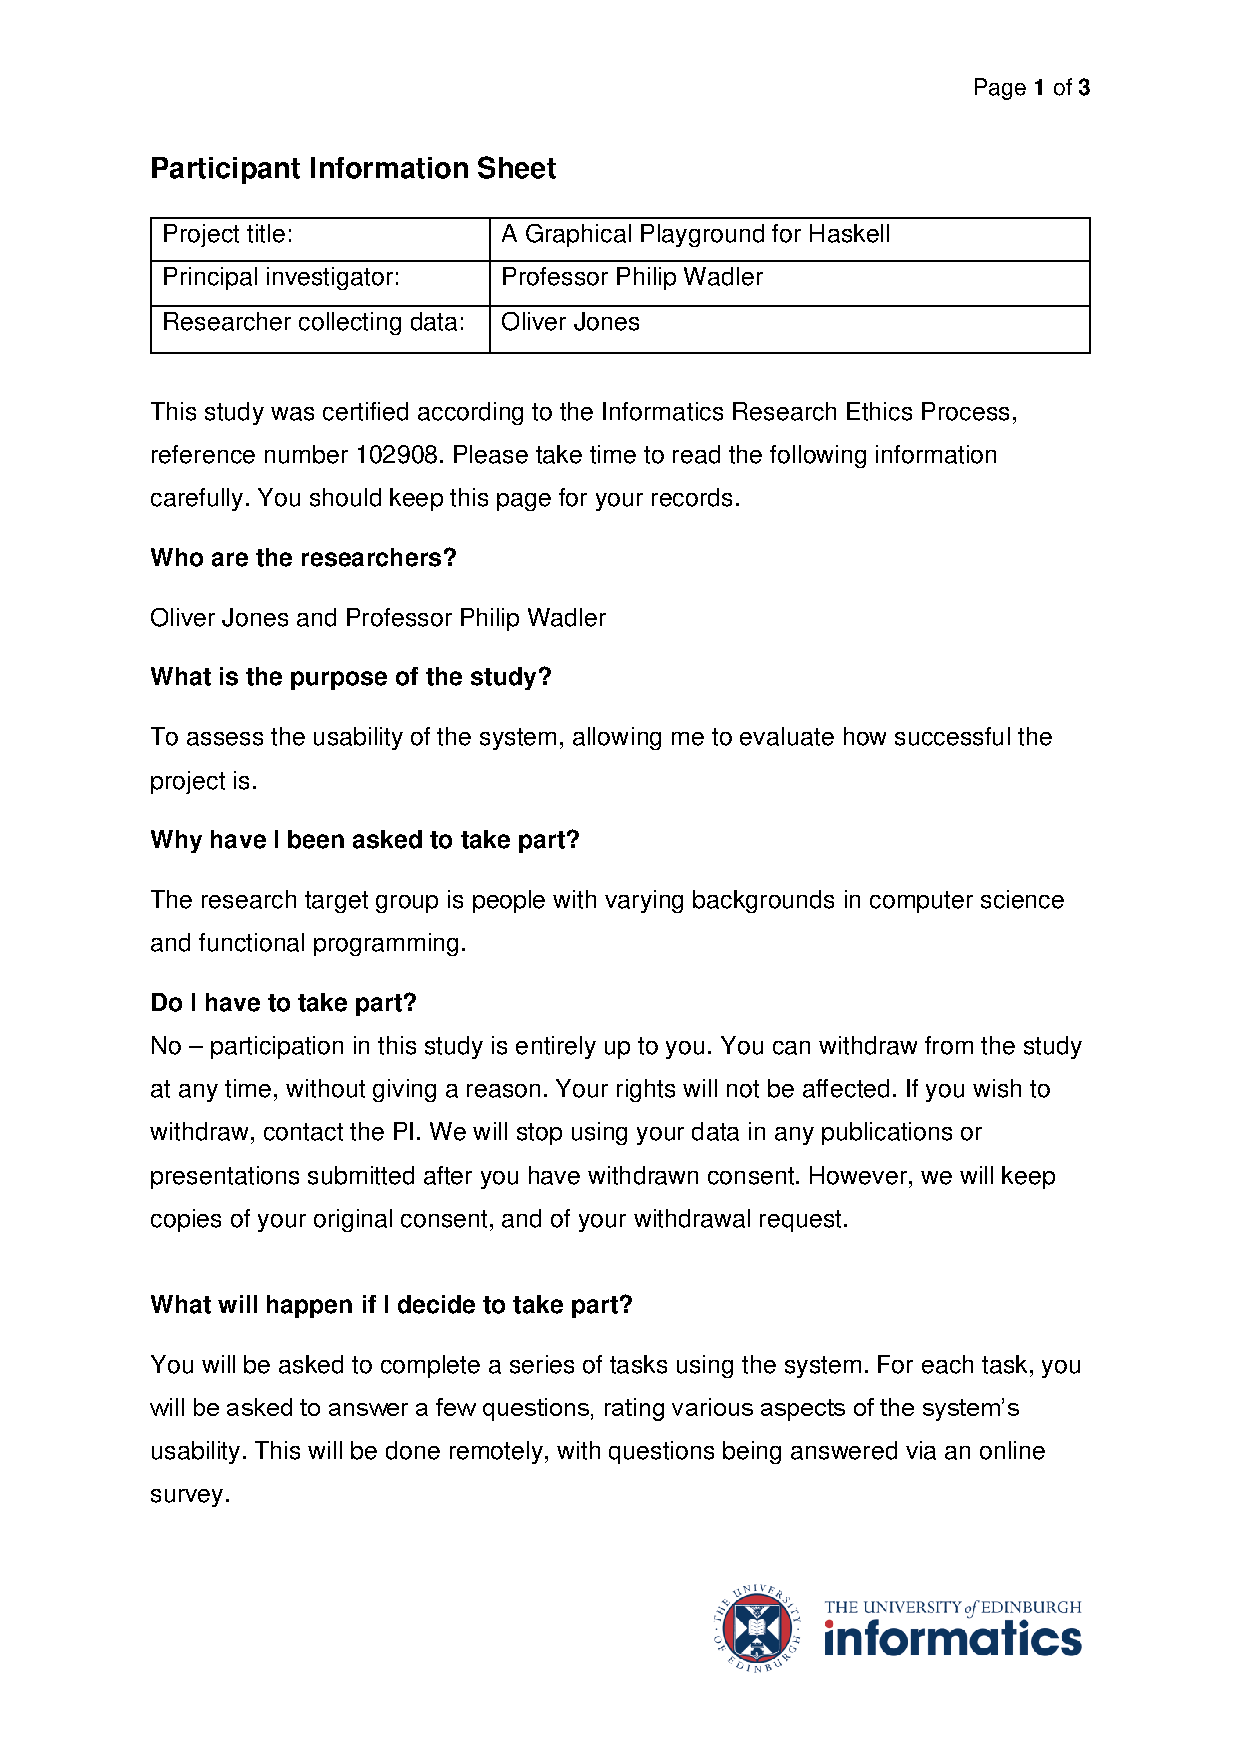
\includepdf[pages=-]{participant-information.pdf}
        \end{center}

    \chapter{Responses to User Testing \& Feedback Survey} \label{app:feedback}
        The following pages contain the responses to the user testing and feedback
            survey, as collected from participants.

    \chapter{Code Listings} \label{app:code}
        The following pages contain the code listings for the graphics library.
        \section*{Lib.hs}
            \lstinputlisting{../public/lib/Lib.hs}
        \section*{Internal.hs}
            \lstinputlisting{../public/lib/Internal.hs}
        \section*{Canvas.hs}
            \lstinputlisting{../public/lib/Canvas.hs}
        \section*{Shape.hs}
            \lstinputlisting{../public/lib/Shape.hs}
        \section*{Maths.hs}
            \lstinputlisting{../public/lib/Maths.hs}
        \section*{Color.hs}
            \lstinputlisting{../public/lib/Color.hs}
\end{document}
